\documentclass[aspectratio=169,11pt]{beamer}
\usepackage{polyglossia}
\setdefaultlanguage{english}
\setotherlanguage{russian}
\usepackage{mathtools}
\usepackage{microtype}
\usepackage{absorbent-theme}
\newfontfamily\cyrillicfontsf{Noto Sans}
\tracinglostchars=3
\title{Absorbent — Your time. Your pace.}
\hypersetup{
  pdftitle={Absorbent — Your time. Your pace.},
  pdfauthor={Ivan Mikhnovich, Egor Zybchenko, Georgy Makarov, Sergey Vazhenin},
  pdfsubject={Multi-Agent Systems — Project Proposal},
  pdfkeywords={Absorbent, lecture notes, multimodal LLM, Project Proposal},
  pdfdisplaydoctitle=true,bookmarksopen=true
}

\begin{document}

% Основные слайды.
\begin{frame}[plain,label=intro]
\pdfbookmark[0]{01 — Your time. Your pace.}{intro}
\darkpalette
\begin{slidecanvas}{PROJECT PROPOSAL\enspace /\enspace 2026}{01 / 08}{1}
  \at{8}{16}{80}{{\fontsize{11}{14}\selectfont\color{mint}Absorbent}}
  \at{8}{25}{86}{{\fontsize{29}{32}\selectfont\bfseries Your time.\\Your pace.}}
  \at{8}{56}{88}{{\fontsize{12}{16}\selectfont Turn lecture recordings\\into illustrated notes.}}
  \at{8}{74}{136}{{\fontsize{6.5}{8.5}\selectfont\color{darkmuted}
    Ivan Mikhnovich\enspace ·\enspace Egor Zybchenko\enspace ·\enspace
    Georgy Makarov\enspace ·\enspace Sergey Vazhenin}}

  % Условный плеер и документ обозначают переход между форматами, не метрики.
  \card{101}{24}{45}{15}{darkpanel}
  \fill[mint] ([xshift=107mm,yshift=-29mm]current page.north west) --
    ++(0,-5mm) -- ++(4mm,2.5mm) -- cycle;
  \foreach \x/\h in {115/2,118/4,121/6,124/3,127/7,130/5,133/3,136/5,139/2}{
    \draw[mint,line width=.65mm,line cap=round]
      ([xshift=\x mm,yshift=-31.5mm]current page.north west) ++(0,-\h mm/2) -- ++(0,\h mm);
  }
  \draw[-{Stealth[length=2mm]},mint,line width=.6mm]
    ([xshift=124mm,yshift=-42mm]current page.north west) -- ++(0,-7mm);
  \card{104}{53}{40}{18}{paper}
  \fill[teal,rounded corners=.5mm]
    ([xshift=109mm,yshift=-57mm]current page.north west) rectangle ++(12mm,-9mm);
  \foreach \y/\w in {57/14,60/17,63/15,66/11}{
    \draw[navy!55,line width=.55mm,line cap=round]
      ([xshift=125mm,yshift=-\y mm]current page.north west) -- ++(\w mm,0);
  }
\end{slidecanvas}
\end{frame}

\begin{frame}[plain,label=demo]
\pdfbookmark[0]{02 — Send a recording}{demo}
\lightpalette
\begin{slidecanvas}{TRY IT LIVE}{02 / 08}{2}
  \at{8}{17}{112}{{\fontsize{23}{27}\selectfont\bfseries Send a recording.\\Get usable material.}}
  \at{8}{42}{108}{{\fontsize{9.5}{12}\selectfont\color{quiet}
    A recording, with optional slides or board photos.}}
  \card{8}{51}{33}{19}{white}
  \at{12}{54}{25}{\smalllabel{01 / SEND}\\[1mm]\textbf{Link or file}}
  \card{45}{51}{33}{19}{white}
  \at{49}{54}{25}{\smalllabel{02 / PROCESS}\\[1mm]\textbf{Absorbent core}}
  \card{82}{51}{33}{19}{white}
  \at{86}{54}{25}{\smalllabel{03 / READ}\\[1mm]\textbf{Illustrated notes}}
  \node[anchor=north west,inner sep=0pt]
    at ([xshift=126mm,yshift=-28mm]current page.north west)
    {\qrcode[height=23mm,hyperlink]{https://t.me/absorbobot}};
  \at{121}{55}{32}{{\fontsize{8}{10}\selectfont\centering
    \href{https://t.me/absorbobot}{\textbf{@absorbobot}}\\
    \color{quiet}Telegram interface}}
  \at{8}{73}{139}{{\fontsize{9}{12}\selectfont\color{teal}
    Start now. Let it process while we explain.}}
\end{slidecanvas}
\end{frame}

\begin{frame}[plain,label=access]
\pdfbookmark[0]{03 — People and AI agents}{access}
\lightpalette
\begin{slidecanvas}{WHY IT MATTERS}{03 / 08}{3}
  \heading{Useful for people.\\Accessible to AI agents.}
  \card{8}{43}{29}{20}{white}
  \at{12}{47}{23}{\textbf{Recording}\\[1mm]{\fontsize{8}{10}\selectfont\color{quiet}Audio / video}}
  \flowarrow{38}{53}{46}{53}
  \card{48}{39}{45}{28}{palegreen}
  \at{52}{43}{37}{\textbf{Text + images}\\[1.5mm]
    {\fontsize{8}{10.5}\selectfont Transcript · keyframes\\Descriptions · notes}}
  \draw[-{Stealth[length=1.7mm]},teal,line width=.5mm]
    ([xshift=95mm,yshift=-53mm]current page.north west) --
    ([xshift=100mm,yshift=-53mm]current page.north west) |-
    ([xshift=105mm,yshift=-43mm]current page.north west);
  \draw[-{Stealth[length=1.7mm]},teal,line width=.5mm]
    ([xshift=100mm,yshift=-53mm]current page.north west) |-
    ([xshift=105mm,yshift=-63mm]current page.north west);
  \at{108}{37}{43}{\textbf{People}\\[1mm]{\fontsize{8.5}{11}\selectfont\color{quiet}Scan. Navigate. Go deeper.}}
  \at{108}{57}{43}{\textbf{AI agents}\\[1mm]{\fontsize{8.5}{11}\selectfont\color{quiet}Use material as a source.}}
  \at{8}{74}{143}{{\fontsize{9.5}{12}\selectfont\color{teal}
    From a time-based medium to material you can work with.}}
\end{slidecanvas}
\end{frame}

\begin{frame}[plain,label=architecture]
\pdfbookmark[0]{04 — Two complementary signals}{architecture}
\lightpalette
\begin{slidecanvas}{HOW IT WORKS}{04 / 08}{4}
  \heading{One recording. Two signals.}
  \at{8}{30}{70}{\smalllabel{SPEECH / EXPLANATION AND LECTURE FLOW}}
  \card{8}{36}{28}{12}{white}
  \at{12}{39}{21}{{\fontsize{9}{11}\selectfont\textbf{Whisper STT}}}
  \flowarrow{37}{42}{42}{42}
  \card{44}{36}{28}{12}{white}
  \at{48}{39}{22}{{\fontsize{9}{11}\selectfont\textbf{Transcript}}}
  \at{8}{55}{46}{\smalllabel{VISUALS / DIAGRAMS AND FORMULAS}}
  \card{8}{61}{28}{12}{white}
  \at{12}{64}{22}{{\fontsize{9}{11}\selectfont\textbf{Keyframes}}}
  \flowarrow{37}{67}{42}{67}
  \card{44}{61}{28}{12}{white}
  \at{48}{64}{22}{{\fontsize{9}{11}\selectfont\textbf{Vision LLM}}}

  \draw[-{Stealth[length=1.5mm]},teal,densely dashed,line width=.4mm]
    ([xshift=58mm,yshift=-49mm]current page.north west) --
    ([xshift=58mm,yshift=-60mm]current page.north west);
  \at{62}{50}{39}{{\fontsize{6.5}{8}\selectfont\color{teal}
    Speech window ±60 s\\+ lecture summary}}
  \draw[-{Stealth[length=1.7mm]},teal,line width=.5mm]
    ([xshift=73mm,yshift=-42mm]current page.north west) --
    ([xshift=105mm,yshift=-42mm]current page.north west) |-
    ([xshift=111mm,yshift=-50mm]current page.north west);
  \draw[-{Stealth[length=1.7mm]},teal,line width=.5mm]
    ([xshift=73mm,yshift=-67mm]current page.north west) --
    ([xshift=105mm,yshift=-67mm]current page.north west) |-
    ([xshift=111mm,yshift=-59mm]current page.north west);
  \card{113}{43}{39}{22}{palegreen}
  \at{117}{47}{32}{\textbf{Notes synthesis}\\[2mm]
    {\fontsize{8}{10}\selectfont MD · HTML · PDF}}
  \at{8}{76}{144}{{\fontsize{7}{9}\selectfont\color{quiet}
    Slides and board photos also enter the vision stage.\quad
    Visual descriptions + synthesis: \texttt{deepseek-flash}.}}
\end{slidecanvas}
\end{frame}

\begin{frame}[plain,label=result]
\pdfbookmark[0]{05 — The actual result}{result}
\lightpalette
\begin{slidecanvas}{SEE THE RESULT}{05 / 08}{5}
  \heading{A readable result — not just a transcript.}
  \at{8}{31}{65}{\smalllabel{SOURCE VIDEO FRAME}}
  \at{81}{31}{71}{\smalllabel{GENERATED NOTES / EARLIER RUN}}
  \node[anchor=north west,inner sep=0pt]
    at ([xshift=8mm,yshift=-36mm]current page.north west)
    {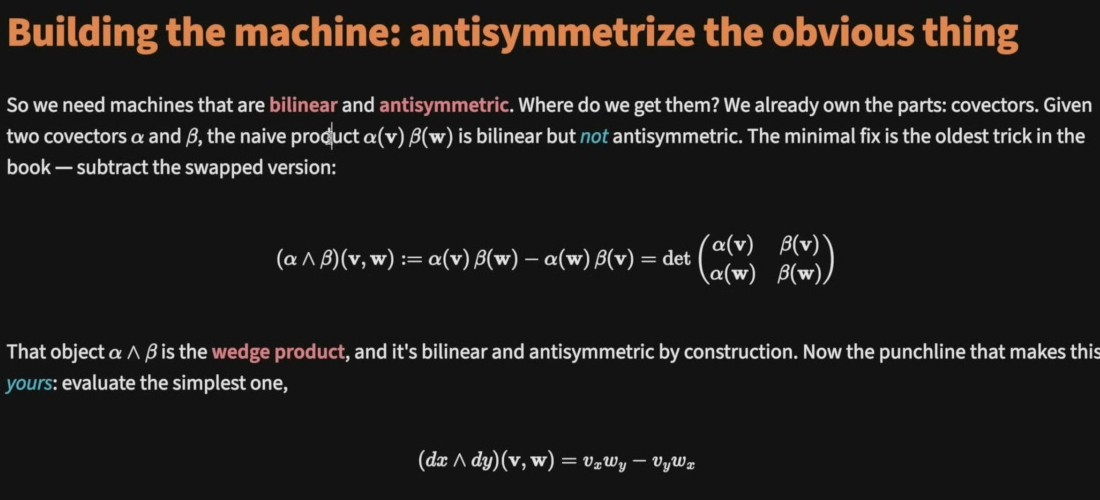
\includegraphics[width=65mm]{assets/source-frame.jpg}};
  \node[anchor=north west,inner sep=0pt]
    at ([xshift=81mm,yshift=-35mm]current page.north west)
    {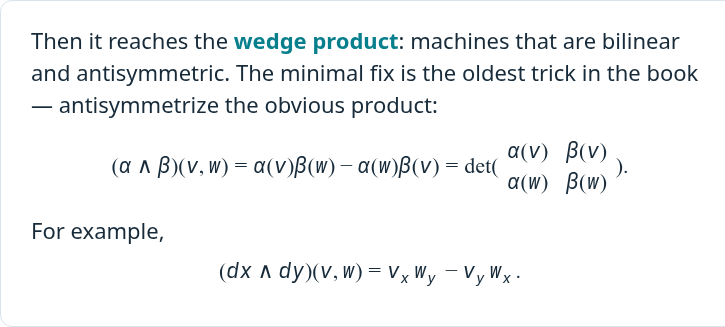
\includegraphics[width=71mm,height=40mm,keepaspectratio]{assets/demo-excerpt.png}};
  \at{8}{75}{143}{{\fontsize{8}{10}\selectfont\color{teal}
    \href{run:demo/notes.html}{Open notes excerpt}\enspace /\enspace
    \href{https://www.youtube.com/watch?v=kzcI5F4tGiU&t=1034s}{Eero Alvar · \textit{How I Use AI to Learn Things} · 17:14}}}
\end{slidecanvas}
\end{frame}

\begin{frame}[plain,label=evaluation]
\pdfbookmark[0]{06 — Evaluation plan}{evaluation}
\lightpalette
\begin{slidecanvas}{EVALUATION PLAN / NOT MEASURED YET}{06 / 08}{6}
  \heading{How we will measure quality.}
  \card{8}{36}{45}{31}{white}
  \at{12}{39}{36}{\smalllabel{01 / COVERAGE}}
  \at{12}{47}{37}{{\fontsize{12}{15}\selectfont\bfseries Key points}}
  \at{12}{55}{36}{{\fontsize{9}{12}\selectfont\color{quiet}Which important ideas\\survive?}}
  \card{57}{36}{45}{31}{white}
  \at{61}{39}{36}{\smalllabel{02 / FAITHFULNESS}}
  \at{61}{47}{37}{{\fontsize{12}{15}\selectfont\bfseries Correct claims}}
  \at{61}{55}{36}{{\fontsize{9}{12}\selectfont\color{quiet}Which claims are\\supported and correct?}}
  \card{106}{36}{46}{31}{white}
  \at{110}{39}{38}{\smalllabel{03 / VISUAL INFORMATION}}
  \at{110}{47}{38}{{\fontsize{12}{15}\selectfont\bfseries Essential visuals}}
  \at{110}{55}{38}{{\fontsize{9}{12}\selectfont\color{quiet}Which formulas and\\diagrams survive?}}
  \at{8}{73}{144}{{\fontsize{8.5}{11}\selectfont\color{teal}
    Compare with transcript-only notes. Same sources. Track time and cost.}}
\end{slidecanvas}
\end{frame}

\begin{frame}[plain,label=readiness]
\pdfbookmark[0]{07 — Working today}{readiness}
\lightpalette
\begin{slidecanvas}{CURRENT STATE}{07 / 08}{7}
  \heading{Working today. Improving next.}
  \card{8}{35}{69}{36}{palegreen}
  \at{13}{39}{59}{{\fontsize{7}{9}\selectfont\bfseries\color{teal}WORKING TODAY}}
  \at{13}{47}{59}{{\fontsize{10}{13}\selectfont
    Audio / video + lecture materials\\[2mm]
    Notes: Markdown / HTML / PDF\\[2mm]
    CLI + separate Telegram bot}}
  \card{83}{35}{69}{36}{white}
  \at{88}{39}{59}{{\fontsize{7}{9}\selectfont\bfseries\color{orange}NEXT / EVIDENCE BEFORE COMPLEXITY}}
  \at{88}{47}{59}{{\fontsize{10}{13}\selectfont
    Establish an evaluation set\\[2mm]
    Compare approaches\\[2mm]
    Improve measured weaknesses}}
  \at{8}{76}{143}{{\fontsize{7.5}{9.5}\selectfont\color{quiet}
    Repository\enspace ·\enspace Dockerfile\enspace ·\enspace
    \texttt{.env.example}\enspace ·\enspace Documented launch}}
\end{slidecanvas}
\end{frame}

\begin{frame}[plain,label=vision]
\pdfbookmark[0]{08 — A foundation for learning agents}{vision}
\darkpalette
\begin{slidecanvas}{THE DIRECTION / NOT A DELIVERY PROMISE}{08 / 08}{8}
  \at{8}{18}{144}{{\fontsize{23}{27}\selectfont\bfseries
    Make recordings useful.\\Then make learning personal.}}
  \card{8}{46}{45}{23}{darkpanel}
  \at{12}{49}{37}{{\fontsize{6.5}{8}\selectfont\bfseries\color{mint}TODAY}}
  \at{12}{56}{37}{{\fontsize{11}{14}\selectfont\bfseries Accessible\\material}}
  \card{57}{46}{45}{23}{darkpanel}
  \at{61}{49}{37}{{\fontsize{6.5}{8}\selectfont\bfseries\color{darkmuted}DIRECTION}}
  \at{61}{56}{37}{{\fontsize{11}{14}\selectfont Source-grounded\\assistance}}
  \card{106}{46}{46}{23}{darkpanel}
  \at{110}{49}{38}{{\fontsize{6.5}{8}\selectfont\bfseries\color{darkmuted}LONG TERM}}
  \at{110}{56}{38}{{\fontsize{11}{14}\selectfont Adaptive\\learning}}
  \at{8}{75}{143}{{\fontsize{8}{10}\selectfont\color{mint}
    \href{https://github.com/multiagent-team/absorbent}{\textcolor{mint}{github.com/multiagent-team/absorbent}}}}
\end{slidecanvas}
\end{frame}

% Резервные слайды открываются только во время вопросов.
\appendix
\begin{frame}[plain,noframenumbering,label=models]
\pdfbookmark[0]{A1 — Models and design choices}{models}
\lightpalette
\begin{slidecanvas}{BACKUP / MODELS AND DESIGN}{A1}{0}
  \heading{Why this pipeline?}
  \at{8}{34}{69}{\smalllabel{THE MODELS}}
  \at{8}{42}{69}{\textbf{Whisper turbo}\\[1mm]
    {\fontsize{9}{12}\selectfont\color{quiet}Local speech recognition.}\\[4mm]
    \textbf{DeepSeek \texttt{deepseek-flash}}\\[1mm]
    {\fontsize{9}{12}\selectfont\color{quiet}Lecture summary, visual descriptions,\\final notes synthesis via API.}}
  \at{86}{34}{65}{\smalllabel{THE CHOICE}}
  \at{86}{42}{65}{{\fontsize{10}{13}\selectfont
    A fixed workflow for a known task.\\[3mm]
    No autonomous tool selection.\\[3mm]
    No training or fine-tuning.}}
  \at{8}{75}{143}{{\fontsize{9}{12}\selectfont\color{teal}
    Add agent autonomy only when it improves an evaluated outcome.}}
\end{slidecanvas}
\end{frame}

\begin{frame}[plain,noframenumbering,label=protocol]
\pdfbookmark[0]{A2 — A fair evaluation protocol}{protocol}
\lightpalette
\begin{slidecanvas}{BACKUP / EVALUATION}{A2}{0}
  \heading{A small, auditable comparison.}
  \at{8}{34}{25}{{\fontsize{22}{25}\selectfont\color{teal}01}}
  \at{28}{35}{121}{\textbf{Annotate the original recording.}\\
    {\fontsize{9}{12}\selectfont\color{quiet}Mark key points and essential visuals; do not treat STT as ground truth.}}
  \at{8}{49}{25}{{\fontsize{22}{25}\selectfont\color{teal}02}}
  \at{28}{50}{121}{\textbf{Compare the same source fragments.}\\
    {\fontsize{9}{12}\selectfont\color{quiet}Transcript-only notes versus the multimodal pipeline. Keep text model fixed.}}
  \at{8}{64}{25}{{\fontsize{22}{25}\selectfont\color{teal}03}}
  \at{28}{65}{121}{\textbf{Audit errors and trade-offs.}\\
    {\fontsize{9}{12}\selectfont\color{quiet}Coverage, unsupported / distorted claims, visual information, time and cost.}}
\end{slidecanvas}
\end{frame}

\begin{frame}[plain,noframenumbering,label=limits]
\pdfbookmark[0]{A3 — Limits and data}{limits}
\lightpalette
\begin{slidecanvas}{BACKUP / LIMITS AND DATA}{A3}{0}
  \heading{What we do not guarantee.}
  \at{8}{35}{38}{{\fontsize{10}{13}\selectfont\bfseries\color{orange}Perfect recognition}}
  \at{53}{35}{98}{{\fontsize{9.5}{12.5}\selectfont STT can distort speech or hallucinate.\\Errors can propagate into the notes.}}
  \at{8}{50}{38}{{\fontsize{10}{13}\selectfont\bfseries\color{orange}Verified facts}}
  \at{53}{50}{98}{{\fontsize{9.5}{12.5}\selectfont Grounding instructions are not a proof.\\No automatic audit of every claim yet.}}
  \at{8}{65}{38}{{\fontsize{10}{13}\selectfont\bfseries\color{orange}Cloud-free defaults}}
  \at{53}{65}{98}{{\fontsize{9.5}{12.5}\selectfont Transcripts and images reach DeepSeek.\\Optional cloud STT sends audio to Mistral.}}
\end{slidecanvas}
\end{frame}

\end{document}
